\documentclass[12pt,a4paper,titlepage]{article}
\usepackage{lab_style}
\usepackage{pdfpages}
\usepackage{eso-pic}
\usepackage{graphicx}
\usepackage{float}
\newcommand\tab[1][1cm]{\hspace*{#1}}

\graphicspath{ {./} }
  
\begin{document}

\begin{titlepage}
\selectlanguage{english}

%----------------------------------------------------------------------------------------
% TITLE PAGE INFORMATION
%----------------------------------------------------------------------------------------
  \begin{center} % Center everything on the page

  %----------------------------------------------------------------------------------------
  % HEADING SECTIONS
  %----------------------------------------------------------------------------------------
  \textsc{\large Faculty of Computers, Informatics and Microelectronics}\\[0.5cm]
  \textsc{\large Technical University of Moldova}\\[1.2cm] % Name of your university/college
  \vspace{25 mm}

  \textsc{\Large Object-Oriented Modeling and Analysis}\\[0.5cm] % Major heading such as course name
  \textsc{\large Laboratory work \#3}\\[0.5cm] % Minor heading such as course title

\newcommand{\HRule}{\rule{\linewidth}{0.5mm}} % Defines a new command for the horizontal lines, change thickness here

  %----------------------------------------------------------------------------------------
  % TITLE SECTION
  %----------------------------------------------------------------------------------------
  \vspace{10 mm}
  \HRule \\[0.4cm]
  { \LARGE \bfseries Sequence Diagrams. Functional and Non-Functional Require-
ments. Conceptual Object Oriented Analysis. Technical Object Oriented Design. }\\[0.4cm] % Title of your document
  \HRule \\[1.5cm]

  %----------------------------------------------------------------------------------------
  % AUTHOR SECTION
  %----------------------------------------------------------------------------------------
      \vspace{30mm}

      \begin{minipage}{0.4\textwidth}
      \begin{flushleft} \large
      \emph{Author:}\\
      Cernei \textsc{Liviu}
      \end{flushleft}
      \end{minipage}
      ~
      \begin{minipage}{0.4\textwidth}
      \begin{flushright} \large
      \emph{Supervisor:} \\
      Mihail \textsc{Gavrilița} % Supervisor's Name
      \end{flushright}
      \end{minipage}\\[4cm]

      \vspace{5 mm}
      % If you don't want a supervisor, uncomment the two lines below and remove the section above
      %\Large \emph{Author:}\\
      %John \textsc{Smith}\\[3cm] % Your name

      %----------------------------------------------------------------------------------------
      % DATE SECTION
      %----------------------------------------------------------------------------------------

      {\large Chișinau 2018}\\[3cm] % Date, change the \today to a set date if you want to be precise

      %----------------------------------------------------------------------------------------
      % LOGO SECTION
      %----------------------------------------------------------------------------------------

      %\includegraphics{red}\\[0.5cm] % Include a department/university logo - this will require the graphicx package

      %----------------------------------------------------------------------------------------

      \vfill % Fill the rest of the page with whitespace
      \end{center}
      
\end{titlepage}

\cleardoublepage

\newpage

\pagenumbering{arabic}
\setcounter{page}{1}
\setcounter{secnumdepth}{4}

\addtocontents{toc}{\protect\thispagestyle{empty}} % no page number on the table of contents page
\cleardoublepage


\phantomsection
\addcontentsline{toc}{section}{Introduction}
\section*{Laboratory work \#3}
\phantomsection

\section{Tasks}
\begin{itemize}
	\item
	Model your application using 3 Sequence Diagrams;
	\item 
	Analyze the Functional and Non-Functional Requirements for your project (at least
5 of each).
\end{itemize}

\section{Theory}

\subsection{Object-Oriented Analysis}
\begin{enumerate}  
	\item Elicit requirements: Define what does the software need to do, and what’s the problem the software trying to solve.
	\item Specify requirements: Describe the requirements, usually, using use cases (and scenarios) or user stories.
	\item Conceptual model: Identify the important objects, refine them, and define their relationships and behavior and draw them in a simple diagram.
\end{enumerate}


\subsection{Conceptual Model}
\begin{enumerate}  
	\item Identifying Objects
	\item Refining Objects
	\item Drawing Objects
	\item Identifying Object Relationships
	\item Identifying Object Behaviors
\end{enumerate}
\clearpage

\section{Sequence Diagrams}
In Figure ~\ref{fig:login} is represented the sequence diagram for the login operation.
\begin{figure}[H]
	\centering
	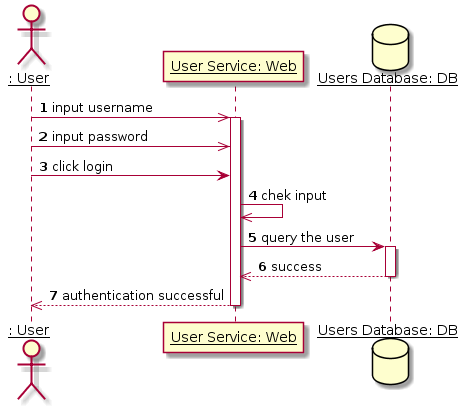
\includegraphics[width=\textwidth]{login}
	\caption{Login sequence diagram}
	\label{fig:login}
\end{figure}
We observe the sequence of operations needed to login any user: student, teacher, or even admin. It is a generalized operation, thats why I used an anonymous calss. The user inputs username and password, the user service check it and sends the information further to the database. The database returns an "success" message, which is propagated to the user by the service. This is the case when all information was correct, and results with the user authenticated.\par

In Figure ~\ref{fig:create} is represented the sequence diagram for creation of a new course.
\begin{figure}[H]
	\centering
	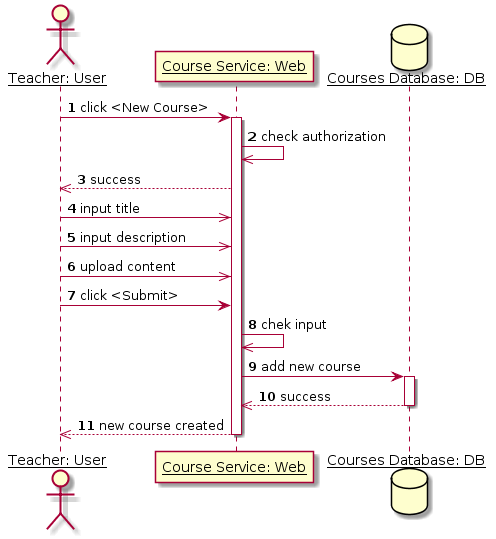
\includegraphics[width=\textwidth]{create}
	\caption{New course sequence diagram}
	\label{fig:create}
\end{figure}
This diagram is specifically for the teacher. In order to create a course, the teacher should have assignet a special authorization key. If it is found, he can begin to input the course information. When submitted, it is checked for invalid fields, then it is sent to the course database. In case of success the teacher is announced through the course service.

In Figure ~\ref{fig:feedback} is represented the sequence diagram for giving feedback for a course.
\begin{figure}[H]
\centering
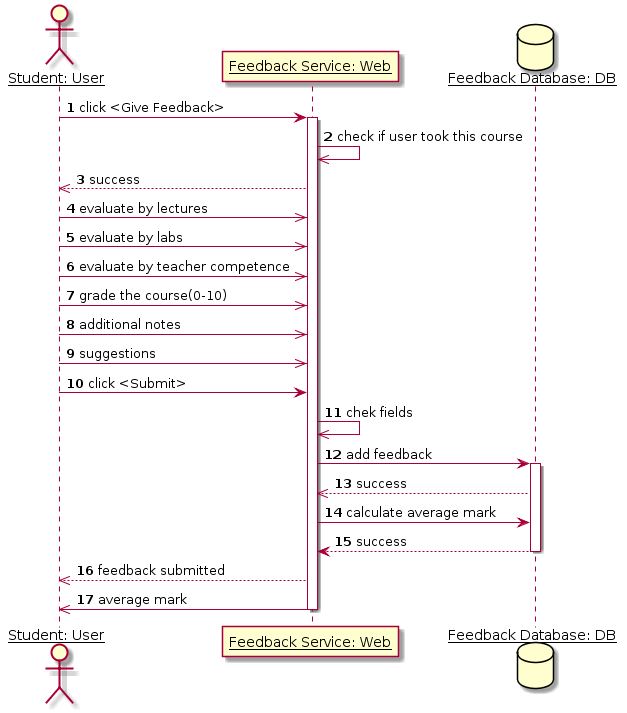
\includegraphics[width=\textwidth]{feedback}
\caption{Feedback sequence diagram}
\label{fig:feedback}
\end{figure}
To be eligible to give feedback, the studnt should have already completed the course. If the condition is satisfied, he can fill the form. After submission, all fields are checked and the information is sent to the database. After a "success" message, the feedback service requests the average mark for that course. Then the student receives an acceptance message and can see the overall quality of the course.

\section{Functional and Non-Functional Requirements}
\subsection{Functional}
\begin{itemize}
	\item Provide access to courses
	\item Teachers can create new courses
	\item Students can take tests
	\item Students can give feedback
	\item Teachers can invite and enroll students
\end{itemize}
\subsection{Non-Functional}
\begin{itemize}
	\item The site supports multiple users at the same time
	\item The information is stored and encripted safely
	\item The site provides very fast access to data
	\item The site can provides access in multiple countries.
	\item The information is processed real-time.
\end{itemize}
\section{Conclusion}
In this laboratory work we learned to create sequence diagrams and write functional and non-functional requirements.

\clearpage
\cleardoublepage

\end{document}
